\section{绪论}
正文是学位论文的主体,第一章为绪论,最后一章为结论与展望。我们来测试一个上标引用。为什么要写这篇论文\footnote{和谐},要解决什么问题,主要观点是什么。 对本论文研究主题范围内已有文献的评述(包括与课题相关的历史的回顾,资料来源、性质及运用情况等)。说明本论文所要解决的问题,所采用的研究手段、方式、方法。明确研究工作的界限和规模。概括论文的主要工作内容。

我们其实已经不知不觉地到达了终点。不幸的是,我们经过20 多
年辛苦跋涉所到达的这个终点,并不是什么美丽的“新世界”,而是中国历史上反复出现过的旧朝代的翻版。王亚南\footnote{中国人}先生早在半个世纪之前就在它那部研究中国官僚体系的开山之作中提醒我们,中国源远流长的官僚政治体系有着神奇的亲和力,它可以与任何体制相互融合。它既可以与古老的小农经济,也可以与现代意义上的自由市场或者国家资本主义相结合;它既能够将儒释道汇于一炉,也能够将现代三民主义、法西斯主义杂糅并蓄之后,自成一体。而当今世界的这个主义,那个主义自然同样不在话下。这或许正是中国官僚政治自秦以降,能够绵绵延续
2000年的关键原因。正所谓“2000年之政,秦政也,皆大盗也。
\begin{figure}[H]
\centering
\subfigure[原始图像]{\label{figure:001} 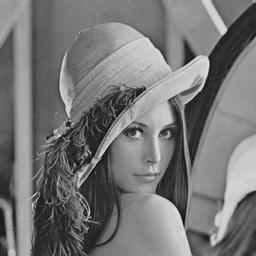
\includegraphics[width=0.2\textwidth]{001}}
\subfigure[噪声图像($\mu=0,\sigma=20$)]{\label{figure:002} 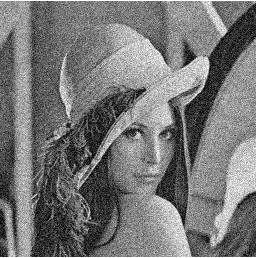
\includegraphics[width=0.2\textwidth]{002}}
\caption{初始图像}
\end{figure}

\begin{figure}[H]
\centering
\subfigure[$\lambda=\frac{1}{20^2}$]{\label{figure:1/20}
 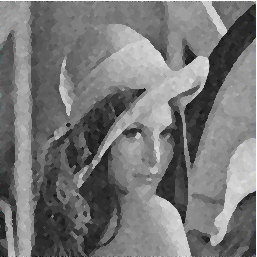
\includegraphics[width=0.2\textwidth]{003}}
\subfigure[$\lambda=\frac{5}{20^2}$]{\label{figure:5/20} 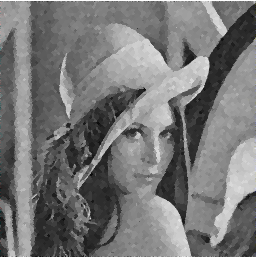
\includegraphics[width=0.2\textwidth]{004}}
\subfigure[$\lambda=\frac{10}{20^2}$]{\label{figure:10/20} 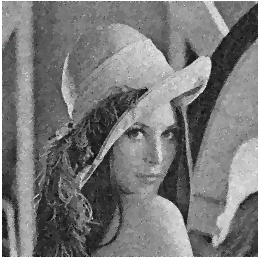
\includegraphics[width=0.2\textwidth]{005}}
\subfigure[$\lambda=\frac{20}{20^2}$]{\label{figure:20/20} 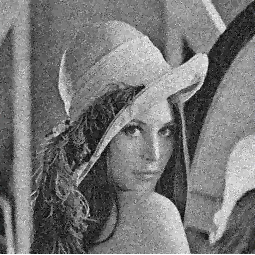
\includegraphics[width=0.2\textwidth]{006}}
\caption{处理的像}
\end{figure}   

    每章标题按一级标题编排,每节标题按二级标题编排,每小节标题按三级标题编排。
    
\subsection{参考文献}
\label{sec:bib}
当然参考文献可以直接写~bibitem,虽然费点功夫,但是好控制,各种格式可以自己随意改
写。

本模板推荐使用~BIB\TeX,样式文件为~thubib.bst,基本符合学校的参考文献格式(如专利
等引用未加详细测试)。看看这个例子,关于书的
\cite{tex, companion, ColdSources},
还有这些 \cite{Krasnogor2004e, clzs, zjsw},关于杂志的\cite{ELIDRISSI94,
  MELLINGER96, SHELL02},硕士论文 \cite{zhubajie, metamori2004},博士论文 \cite{shaheshang, FistSystem01},标准文件\cite{IEEE-1363},会议论文 \cite{DPMG,kocher99},技术报告\cite{NPB2}。中文参考文献\cite{cnarticle}应增~\texttt{lang=``zh''}~字段,以便进行相应处理。另外,这个~bst 对中文文献\cite{cnproceed}的支持并不是十全十美,如果有不如意的地方,请手动修改~bbl 文件。

    \begin{table}[htb]
  \centering
  \begin{minipage}[t]{1\linewidth} 
  % 如果想在表格中使用脚注,minipage是个不错的办法
  \caption[模板文件]{模板文件。如果表格的标题很长,那么在表格索引中就会很不美
    观,所以要像~chapter 那样在前面用中括号写一个简短的标题。这个标题会出现在索
    引中。}
  \label{tab:template-files}
    \begin{tabular*}{\linewidth}{lp{10cm}}
      \toprule[1.5pt]
      {\bf文件名} & {\bf 描述} \\\midrule[1pt]
      thuthesis.ins & \LaTeX{} 安装文件,docstrip\footnote{表格中的脚注} \\
      thuthesis.dtx & 所有的一切都在这里面\footnote{再来一个}。\\
      thuthesis.cls & 模板类文件。\\
      thuthesis.cfg & 模板配置文。cls 和~cfg 由前两个文件生成。\\
      thubib.bst    & 参考文献~Bibtex 样式文件。\\
      thutils.sty   & 常用的包和命令写在这里,减轻主文件的负担。\\
      \bottomrule[1.5pt]
    \end{tabular*}
  \end{minipage}
\end{table}

    “章”、“节”、“小节”的编号统一为:1、1.1、1.1.1。
    
\begin{equation}
\frac{x}{y}
\end{equation}


    四级以后的标题和编号的编排原则\footnote{是什么}为:下级标题的显目程度不超过上一级,不重复或混淆。

    编号与题目之间空一格。

    \subsection{二级标题}
    

        积土成山,风雨兴焉;积水成渊,蛟龙生焉;积善成德,而神明自得,圣心备焉。故不积跬步,无以至千里;不积小流,无以成江海。骐骥一跃,不能十步;驽马十驾,功在不舍。锲而舍之,朽木不折;锲而不舍,金石可镂。蚓无爪牙之利,筋骨之强,上食埃土,下饮黄泉,用心一也。蟹六跪而二螯,非蛇鳝之穴无可寄托者,用心躁也。
         

        \subsection{三级标题}

        平林漠漠烟如织,寒山一带伤心碧。暝色入高楼,有人楼上愁。王阶空伫立,宿鸟归飞急。何处是归程,长亭更短亭。


            \subsubsection{四级标题}
                
            君不见,黄河之水天上来,奔流到海不复回。君不见,高堂明镜悲白发,朝如青丝暮成雪。人生得意须尽欢,莫使金樽空对月。天生我材必有用,千金散尽还复来。烹羊宰牛且为乐,会须一饮三百杯。岑夫子,丹丘生,将进酒,君莫停。与君歌一曲,请君为我侧耳听。钟鼓馔玉不足贵,但愿长醉不复醒。古来圣贤皆寂寞,惟有饮者留其名。陈王昔时宴平乐,斗酒十千恣欢谑。主人何为言少钱,径须沽取对君酌。五花马,千金裘,呼儿将出换美酒,与尔同销万古愁。

            \subsubsection{四级标题}

                一屠晚归,担中肉尽,止有剩骨。途中两狼,缀行甚远。

                屠惧,投以骨。一狼得骨止,一狼仍从。复投之,后狼止而前狼又至。骨已尽矣,而两狼之并驱如故。

                屠大窘,恐前后受其敌。顾野有麦场,场主积薪其中,苫蔽成丘。屠乃奔倚其下,弛担持刀。狼不敢前,眈眈相向。

                少时,一狼径去,其一犬坐于前。久之,目似瞑,意暇甚。屠暴起,以刀劈狼首,又数刀毙之。方欲行,转视积薪后,一狼洞其中,意将隧入以攻其后也。身已半入,止露尻尾。屠自后断其股,亦毙之。乃悟前狼假寐,盖以诱敌。

                狼亦黠矣,而顷刻两毙,禽兽之变诈几何哉?止增笑耳。

            \subsubsection{又是一个四级标题}

                孔子东游,见两小儿辩斗。问其故。

                一儿曰:“我以日始出时去人近,而日中时远也。”

                一儿以日初出远,而日中时近也。

                一儿曰:“日初出大如车盖,及日中则如盘盂,此不为远者小而近者大乎?”

                一儿曰:“日初出沧沧凉凉,及其日中如探汤,此不为近者热而远者凉乎?”

                孔子不能决也。

                两小儿笑曰:“孰为汝多知乎?”

